\section{Method}
% General

% 
In this section, we propose a framework for social-aware driving scenario generation. First, we introduce VLMs for high level scenario analysis and social interaction proposal. Second, we propose a reward integration module to judge the reward of a vehicle, which is also capable of depicting the different social personality of drivers. Third, we guide a multi-agent diffusion model for joint trajectory generation. 

% \begin{figure}[htbp]
%     \centering
%     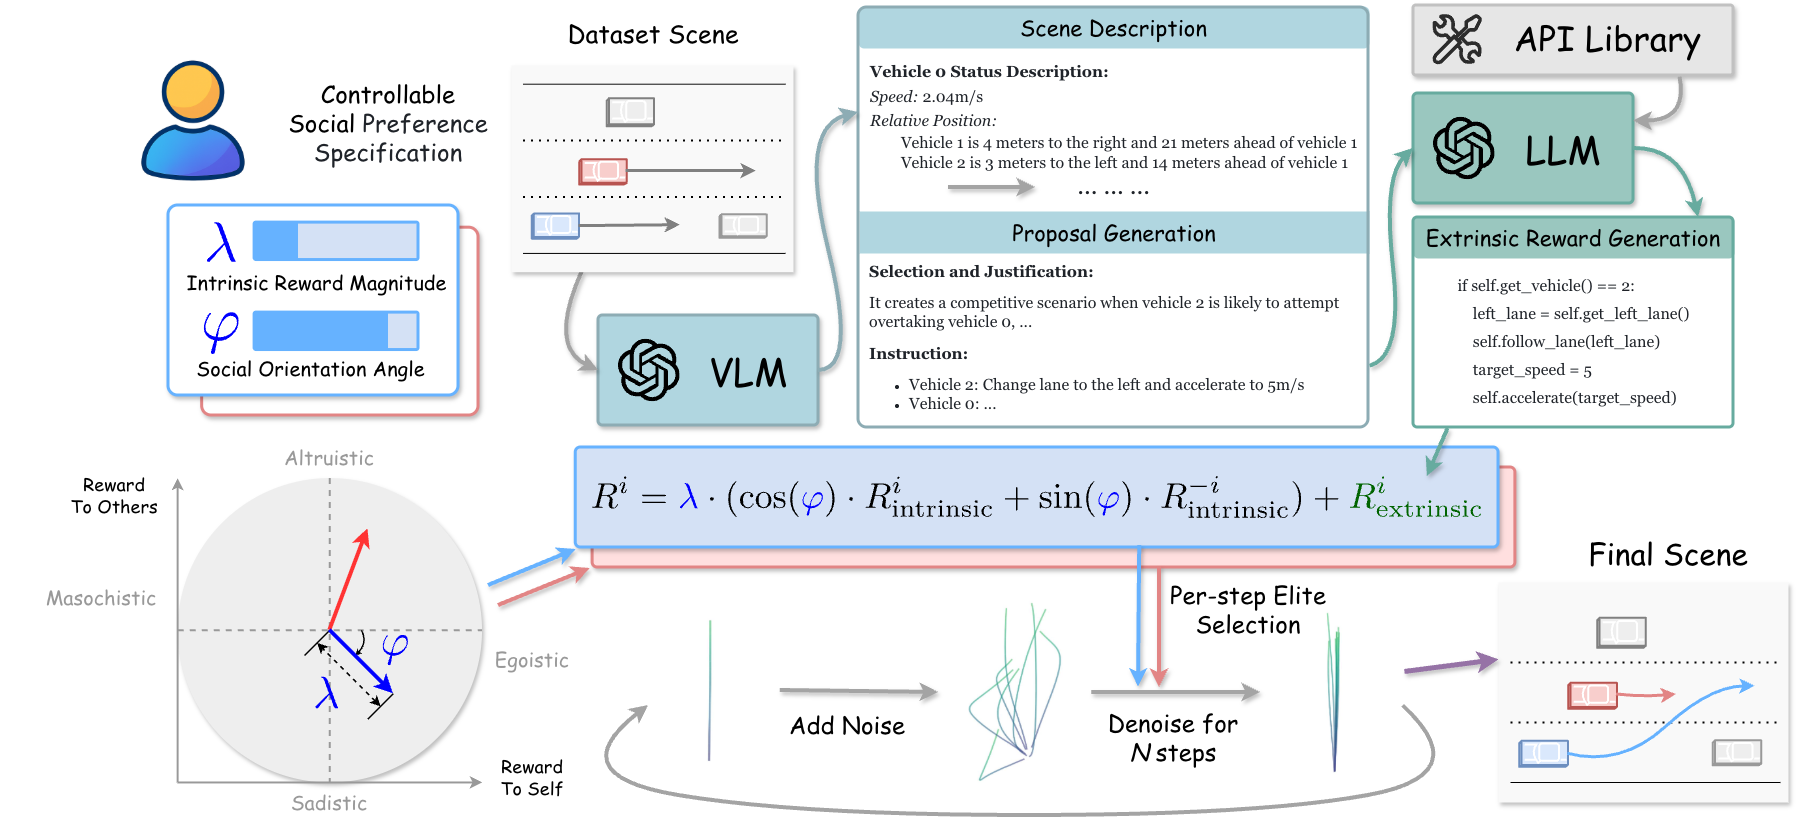
\includegraphics[width=1.0\textwidth]{figures/changan_new.drawio.png}
%     \caption{Overview of \our. The framework leverages VLMs and LLMs to construct social rewards that guide a multi-agent diffusion process.}
%     \vspace{-8pt}
%     \label{fig:social-drive-gen}
% \end{figure}

\subsection{Scenario Analysis and Proposal Generation with VLM}

We leverage Visual-Language Models (VLMs) to identify and generate adverserial interactive scenario proposals from real-world driving datasets. The process is executed in two distinct stages:

\textbf{Semantic Scene Description Stage} We define the state of a single vehicle $i$ at time $t$ be denoted by a vector $\mathbf{s_t^i}=[p_t^i,v_t^i,\theta_t^i]$, representing its position, velocity, and heading. A vehicle's trajectory is thus a sequence of states, $\tau_i=\{s_1^i,s_2^i,\dots ,s_{T_s}^i\}$, where $T_s$ is the total duration of the traffic. The entire scenario, extracted from a real-world dataset, is represented as a tuple $\mathcal{S}=(\cup_{i=1}^N \tau_i,\mathcal{M})$, where $N$ is the total number of vehicles and $\mathcal{M}$ denotes the visual map data. By analyzing the state $S$, the VLM generates a natural language description $D_{\text{scene}}= \text{VLM}(\mathcal{S})$ that captures the scene's dynamic features including relative spatial positions, relative speed and infers underlying social intentions. 

\textbf{Adversarial Proposal Generation Stage} Subsequently, the VLM acts as a strategic proposer. Conditioned on the scene description $D_{\text{scene}}$ and visual map data $\mathcal{M}$, it selects a pair of vehicles $\{v_i,v_j\}$ from the set of all vehicles with the highest potential for social interaction. It is prompted to generate specific, human-like adversarial proposals, $\mathcal{P}_{i, j} = \{\mathcal{A}_i, \mathcal{A}_j\}$, for these two vehicles. Here, $\mathcal{A}_i$ and $\mathcal{A}_j$  are natural language instructions that specify high level intentions corresponding to vehicles $v_i$ and $v_j$. For \our,  $\mathcal{P}_{i, j}$ serve as critical conditioning signals for the downstream trajectory generation process, ensuring that the final generated scenarios are highly interactive and diverse.

\subsection{Social-aware Reward Formulation}

To achieve the simulation of varied driving scenarios, we design a social-aware reward function inspired by established social psychological theories and their extensions. This function evaluates driving behaviors and guides the downstream generative model to generate scenarios across a broad spectrum of game-theoretic interactions, from cooperative to highly adversarial.

\subsubsection{Decomposition of Social Behavior} 

To achieve a more nuanced representation of driving behavior, we decompose social motivation along two critical axes, addressing key limitations in recent literature. 

First, prior works~\citep{schwarting2019social, dai2023socially} often represent Social Value Orientation (SVO) on a 1D spectrum. These approaches conflate distinct motivations—such as a reckless agent (low concern for self, low concern for others) and a purely selfish agent (high concern for self, low concern for others)—into a single ambiguous value. More fundamentally, these models often incorrectly assume the scope of social preference. They implicitly define the SVO of an agent $i$ as applying to the entirety of another's reward, $R_{-i}$, which conflates the other's intrinsic values (e.g., safety, comfort) with their extrinsic, task-specific goals, $R_{-i}^{\text{extrinsic}}$. This is unrealistic, since the extrinsic motivation or task-goal of another vehicle is generally unobservable to the driver. Therefore, a driver's social preference (e.g., altruism) can realistically only apply to the other's inferred intrinsic values, such as their safety and comfort, not their specific, hidden goals.

\subsubsection{The Integrated Reward Function} 

Building on the dual decomposition from the previous section, we now formalize the integrated reward function for agent $i$. The total reward $R_i$ is composed of two primary components: a social-aware intrinsic term and a task-oriented extrinsic term.

These components are balanced by a intrinsic reward magnitude $\lambda$, which controls the agent's tendency to pursue extrinsic goals versus intrinsic values. The intrinsic term itself is governed by a social orientation angle $\phi$, which sets the agent's SVO angle. This is formulated as:

\begin{equation} \label{eq:social_reward}
R_i = \lambda \cdot ( \cos(\phi) \cdot R^{i}_{\text{intrinsic}} + \sin(\phi) \cdot R^{-i}_{\text{intrinsic}}) + R^{i}_{\text{extrinsic}}
\end{equation}

The \textbf{extrinsic reward} ($R_{\text{extrinsic}}$) is dynamically generated by the LLM to be task-oriented. Based on the natural language proposal $\mathcal{P}_{i,j}$ from the previous stage generated by the VLM, the LLM parses the specific objective (e.g., "successfully complete a lane change") and invokes a predefined reward API to instantiate a concrete reward function. This design makes our framework highly extensible, allowing it to adapt to diverse adversarial proposals. In contrast, the \textbf{intrinsic rewards} ($R_{\text{intrinsic}}$) are internally motivated, reflecting the inherent preferences of the driver. $R_{\text{intrinsic}}$ accounts for a driver's personal comfort, safety, and adherence to standard driving rules, including lane keeping, speed maintenance, and heading consistency.

\subsection{Multi-vehicle Trajectory Generation} 

The downstream generation module of \our generates multi-agent trajectories that maximize the social-aware reward functions defined in the previous section. Our approach adapts the Evolutionary Strategy (ES)-guided diffusion model~\citep{yang2024diffusion} to a multi-agent setting. Unlike prior work that typically applies reward guidance only to the final denoised output, our method integrates this guidance throughout the entire denoising process. 


\subsubsection{Denoising Process with Step-wise Guidance} Our key innovation is to integrate a reward-based evolutionary search into each iterative denoising step, progressively refining trajectories toward high-reward solutions.

Given a trained diffusion model, a standard reverse diffusion process for a single step can be expressed as: 
\begin{equation} p_\theta(\mathbf{x}_{t-1}|\mathbf{x}_t) = \mathcal{N}(\mathbf{x}_{t-1}; \boldsymbol{\mu}_\theta(\mathbf{x}_t, t), \boldsymbol{\Sigma}_\theta(\mathbf{x}_t, t)) \end{equation}
 where $x_t$ is a noisy sample at timestep $t$, and the model $\theta$ predicts the mean $\mu$ and covariance $\Sigma$ to generate a less noisy sample $\mathbf{x}_{t-1}$.

Our method introduces a gradient-free evolutionary guidance loop that leverages our reward function. This process begins with an initial population of $M$ trajectories. At each search step $k$, the entire population is renoised to promote exploration. The core of our guidance then occurs within the inner denoising loop. At each denoising step $t$, we first evaluate the entire noisy population $\mathbf{X}_t$. For each noisy sample $\mathbf{x}_t^{(i)}$, we predict its corresponding clean trajectory $\mathbf{x}_0^{(i)}$ and evaluate its reward, $R(\mathbf{x}_0^{(i)})$. This reward is then assigned back to  $\mathbf{x}_t^{(i)}$.

A reward-weighted "elite" distribution $q$ is then computed over this noisy population $\mathbf{X}_t$, formally defined as:
\begin{equation}
q(\mathbf{x}) = \frac{\exp(\tau \cdot R(\mathbf{x}))}{\sum_{j=1}^{M} \exp(\tau \cdot R(\mathbf{x}_t^{(j)}))}
\end{equation}
where $\tau$ is the temperature parameter. This distribution $q$ is then used to sample a population of ``elites" from $\mathbf{X}_t$, which forms the basis for the subsequent denoising step $t-1$. This step-wise selection loop continuously guides the generation process, progressively refining the trajectories toward high-reward solutions.

Crucially, the temperature parameter $\tau$ is not fixed. We employ an annealing schedule for $\tau$, increasing its value as the denoising process progresses. This strategy enables an exploratory search in the early stages when noise is high, and transitions to an exploitative search in the later stages when the trajectories are more refined. This approach balances exploration (diversity) with exploitation (high-reward solutions).

\subsubsection{Joint Multi-Agent Trajectory Generation}
We extend the single-agent diffusion framework to a multi-agent setting by modeling the joint trajectory distribution of all vehicles. Unlike individual generation, this approach explicitly captures inter-agent dependencies. By guiding this joint process with a social-aware reward function, we optimize the entire interactive scenario to align with high-level adversarial proposals. This ensures that collective behaviors are not only cohesive and physically plausible but also conform to the desired game-theoretic outcomes.


% \begin{algorithm}[H]
%     \caption{Reward Guided Trajectory Generation}
%     \label{alg:traj_gen}
%     \begin{algorithmic}[1]
%         \Require Diffusion model $p_\theta$, reward function $R$, number of search steps $K$, population size $M$, number of denoising steps $N$, variance schedule $\bar{\alpha} = \{\bar{\alpha}_i\}_{i=1}^{N}$.
%         \State Initialize population $\mathbf{X}^0 \leftarrow \{x_i \sim p_\theta(x)\}_{i=1}^M$
%         \For{search step $k = 1, \dots, K$}
%             \State Renoise population: 
%             \State \hspace{\algorithmicindent}$\mathbf{\bar{E}}_k \leftarrow \{ \sqrt{\bar{\alpha}_N} x + \sqrt{1 - \bar{\alpha}_N} \epsilon \mid x \in \mathbf{X}^{k-1},\,\epsilon \sim \mathcal{N} (0, 1) \}$
%             % \State Compute distribution $q(\mathbf{x}) = \frac{\exp(\tau \cdot R(\mathbf{x}))}{\sum_{j=1}^M \exp(\tau \cdot R(\mathbf{x}_j))}$
%             % \State Sample elite population $\mathbf{E}_k \leftarrow \{\mathbf{x}_i \sim q(\mathbf{x})\}_{i=1}^M$
%             \State Denoise elites $\mathbf{E}_k \leftarrow \text{DenoiseAndSample}(\mathbf{\bar{E}}_k,\,p_{\theta},\,R,\,N, M) $
%             \State Set new population $\mathbf{X}^k \leftarrow \mathbf{E}_k$
%         \EndFor
%         \State \Return $\arg\max_{x \in \mathbf{X}^K} R(x)$
%     \end{algorithmic}
% \end{algorithm}

% \begin{algorithm}[H]
%     \caption{Step-wise Evolutionary Denoising}
%     \label{alg:denoise_sample}
%     \begin{algorithmic}[1]
%         \Require Noise population $\mathbf{X_{\text{noise}}}$, diffusion model $p_{\theta}$, reward function $R$, number of denoising steps $N$, population size $M$. 
%         \Function{DenoiseAndSample}{$\mathbf{x}_{\text{noise}}$, $p_{\theta}$, $R$, $N$, $M$}
%             \State Set current noise population $\mathbf{X}_N \leftarrow \mathbf{X}_{\text{noise}}$
%             \For{denoising step $t = N, \dots, 1$}
%                 % \State Denoise samples $\mathbf{X}_{\text{clean}} \leftarrow \{\mathbf{x}_{t-1} \sim p_{\theta} (\mathbf{x}_{t-1} \mid \mathbf{x}_t) \mid \mathbf{x}_t \in \mathbf{X}^t\}$
%                 \ForAll{$x_t^{(i)} \in X_{t}$}
%                 \State Predict a clean sample by fully denoising:
%                 \State \hspace{\algorithmicindent} $x_0^{(i)} \leftarrow p_{\theta}(x|x_t^{(i)})$
%                 \State Assign reward to the corresponding noise sample:
%                 \State \hspace{\algorithmicindent} $R(x_t^{(i)}) \leftarrow R(x_0^{(i)})$
%                 \EndFor
                
%                 % \State Denoise samples $\mathbf{X}_{\text{clean}} \leftarrow \{\mathbf{x} \sim p_{\theta} (\mathbf{x} | \mathbf{x}_t) \mid \mathbf{x}_t \in \mathbf{X}^t\}$
%                 % \State Compute rewards $\{R(x) \mid x \in \mathbf{X}_{\text{clean}}\}$
%                 \State Compute distribution $q(x) = \frac{\exp(\tau \cdot R(x))}{\sum_{x_t^{(j)} \in \mathbf{X}_{t}} \exp(\tau \cdot R(x_t^{(j)}))}$
%                 \State Sample next population $\mathbf{X}_{t-1} \leftarrow \{{x}_{t-1} \overset{\mathrm{iid}}{\sim} q(x)\}_{i=1}^M$
%             \EndFor
%             \State \Return $\mathbf{X}_0$
%         \EndFunction
%     \end{algorithmic}
% \end{algorithm}


% \begin{algorithm}[H]
%     \caption{Multi-Agent Trajectory Generation}
%     \label{alg:traj_gen}
%     \begin{algorithmic}[1]
%         \Require Diffusion model $p_\theta$, reward function $R$, number of search steps $K$, population size $M$, number of denoising steps $N$, variance schedule $\bar{\alpha} = \{\bar{\alpha}_i\}_{i=1}^{N}$.
%         \State Initialize population $\mathbf{X}^0 \leftarrow \{\mathbf{x}_i \sim p_\theta(\mathbf{x})\}_{i=1}^M$
%         \For{search step $k = 1, \dots, K$}
%             \State Renoise population $\mathbf{\bar{E}}_k \leftarrow \{ \sqrt{\bar{\alpha}_N} x + \sqrt{1 - \bar{\alpha}_N} \epsilon \mid x \in \mathbf{X}^{k-1},\,\epsilon \sim \mathcal{N} (0, 1) \}$
%             % \State Compute distribution $q(\mathbf{x}) = \frac{\exp(\tau \cdot R(\mathbf{x}))}{\sum_{j=1}^M \exp(\tau \cdot R(\mathbf{x}_j))}$
%             % \State Sample elite population $\mathbf{E}_k \leftarrow \{\mathbf{x}_i \sim q(\mathbf{x})\}_{i=1}^M$
%             \State Denoise elites $\mathbf{E}_k \leftarrow \text{DenoiseAndSample}(\mathbf{\bar{E}}_k,\,p_{\theta},\,R,\,N)) $
%             \State Set new population $\mathbf{X}^k \leftarrow \mathbf{E}_k$
%         \EndFor
%         \State \Return $\arg\max_{\mathbf{x} \in \mathbf{X}^K} R(\mathbf{x})$
%     \end{algorithmic}
% \end{algorithm}

% \begin{algorithm}[H]
%     \caption{Iterative Guided Denoising}
%     \label{alg:denoise_sample}
%     \begin{algorithmic}[1]
%         \Require Noise population $\mathbf{X_{\text{noise}}}$, diffusion model $p_{\theta}$, number of denoising steps $N$, Reward function $R$. 
%         \Function{DenoiseAndSample}{$\mathbf{x}_{\text{noise}}$}
%             \State Set current noise population $\mathbf{X}_N \leftarrow \mathbf{X}_{\text{noise}}$
%             \For{denoising step $t = N, \dots, 1$}
%                 % \State Denoise samples $\mathbf{X}_{\text{clean}} \leftarrow \{\mathbf{x}_{t-1} \sim p_{\theta} (\mathbf{x}_{t-1} \mid \mathbf{x}_t) \mid \mathbf{x}_t \in \mathbf{X}^t\}$
%                 \ForAll{$x_t^{(i)} \in X_{t-1}$}
%                 \State Predict a clean sample by fully denoising: $x_0^i \leftarrow p_{\theta}(x|x_t^{(i)})$
%                 \State Assign reward to the corresponding noise sample:
%                 \State \hspace{\algorithmicindent} $R_i \leftarrow R(\mathbf{x}_0^{\text{pred}, (i)})$
%                 \EndFor
                
%                 % \State Denoise samples $\mathbf{X}_{\text{clean}} \leftarrow \{\mathbf{x} \sim p_{\theta} (\mathbf{x} | \mathbf{x}_t) \mid \mathbf{x}_t \in \mathbf{X}^t\}$
%                 % \State Compute rewards $\{R(x) \mid x \in \mathbf{X}_{\text{clean}}\}$
%                 \State Compute distribution $q(\mathbf{x}) = \frac{\exp(\tau \cdot R(\mathbf{x}))}{\sum_{\mathbf{x}_t^{(j)} \in \mathbf{X}_{t}} \exp(\tau \cdot R(x_t^{(j)}))}$
%                 \State Sample next population $\mathbf{X}_{t-1} \leftarrow \{\mathbf{x}_{t-1} \overset{\mathrm{iid}}{\sim} q(\mathbf{x})\}$
%             \EndFor
%             \State \Return $\mathbf{X}$
%         \EndFunction
%     \end{algorithmic}
% \end{algorithm}

